\documentclass[a4paper,12pt]{article} 
\usepackage[utf8]{inputenc} % Acentos válidos sin problemas
\usepackage[spanish]{babel} % Idioma
\usepackage{algorithm}
\usepackage{algorithmic}
\usepackage[backend=biber, style=alphabetic, sorting=ynt]{biblatex}
\bibliography{bibliografia.bib}
\nocite{*} % Añade todas las referencias de bib sin cita

%-----------------------------------INICIO DE PACKETES-------------------/
%-----------------------------------------------------------------------/
\usepackage{amsmath}   % Matemáticas: Comandos extras(cajas ecuaciones) |
\usepackage{amsthm}
\usepackage{amssymb}   % Matemáticas: Símbolos matemáticos              |
\usepackage{datetime}  % Agregar fechas                                 |
\usepackage{graphicx}  % Insertar Imágenes                              |
%\usepackage{biblatex} % Bibliografía                                   |
\usepackage{multicol}  % Creación de tablas                             |
\usepackage{longtable} % Tablas más largas                              |
\usepackage{xcolor}    % Permite cambiar colores del texto              |
\usepackage{tcolorbox} % Cajas de color                                 |
\usepackage{setspace}  % Usar espacios                                  |
\usepackage{fancyhdr}  % Para agregar encabezado y pie de página        |
\usepackage{lastpage}  %                                                 |
\usepackage{float}     % Flotantes                                      |
\usepackage{soul}      % "Efectos" en palabras                          |
\usepackage{hyperref}  % Para usar hipervínculos                        |
\usepackage{caption}   % Utilizar las referencias                       |
\usepackage{subcaption} % Poder usar subfiguras                         |
\usepackage{multirow}  % Nos permite modificar tablas                   |
\usepackage{array}     % Permite utilizar los valores para multicolumn  |
\usepackage{booktabs}  % Permite modificar tablas                       |
\usepackage{diagbox}   % Diagonales para las tablas                     |
\usepackage{colortbl}  % Color para tablas                              |
\usepackage{listings}  % Escribir código                               |
\usepackage{mathtools} % SIMBOLO :=                                     |
\usepackage{enumitem}  % Modificar items de Listas                      |
\usepackage{tikz}      %                                                |
\usepackage{lipsum}    % for auto generating text                       |
\usepackage{afterpage} % for "\afterpage"s                              |
\usepackage{pagecolor} % With option pagecolor={somecolor or none}|     |
\usepackage{xpatch}    % Color de lineas C & F
%\usepackage{glossaries} %                                              |
\usepackage{lastpage}    %                                              |   
\usepackage{csquotes}    %                                              |
%-----------------------------------------------------------------------\
%-----------------------------------FIN--- DE PACKETES-------------------\

\usepackage{pgfplots}     %                                             |
\pgfplotsset{compat=1.18} %           
\usepackage{etoolbox}
\usepackage{tikz,times}
\usepackage{verbatim}
\usetikzlibrary{mindmap,trees,backgrounds}
%--------------------------------/
%-------------------------------/
\usepackage[                 %   |
  headheight=15pt,  %            |
  letterpaper,  % Tipo de pag.   |
  left =1.5cm,  %  < 1 >         |
  right =1.5cm, %  < 1 >         | MARGENES DE LA PAGINA
  top =2cm,     %  < 1.5 >       |
  bottom =1.5cm %  < 1.5 >       |
]{geometry}     %                |
%-------------------------------\
%--------------------------------\

%----------------------------------------------------------------------/
%-------------------Encabezado y Pie de Pagina-----------------------/ |
%--------------------------------------------------------------------\ |
%\fancyhf{}
%\pagestyle{fancy}

\fancypagestyle{firstpage}{  
    \fancyhead[L]{}
    \fancyhead[R]{}     
    \fancyfoot[L]{}
    \fancyfoot[C]{}
    \fancyfoot[R]{\thepage\ de \pageref*{LastPage}}    
    \renewcommand{\headrulewidth}{0pt} 
    \xpretocmd\headrule{}{}{\PatchFailed}
}

\fancypagestyle{fancy}{  
    \fancyhead[L]{\textbf{Semestre: 2024-2}}
    \fancyhead[C]{}     
    \fancyhead[R]{}     

    \fancyfoot[L]{\texttt{Skynet Scribes}}
    \fancyfoot[C]{\texttt{IA}}
    \fancyfoot[R]{\thepage\ de \pageref*{LastPage}}

    \renewcommand{\headrulewidth}{1pt} 
    \xpretocmd\headrule{}{}{\PatchFailed}
    \renewcommand{\footrulewidth}{1.5pt} 
    \xpretocmd\footrule{}{}{\PatchFailed}
}

\fancypagestyle{fancyref}{  
    \fancyhead[L]{}
    \fancyhead[R]{}     
    \fancyfoot[L]{\texttt{Skynet Scribes}}
    \fancyfoot[C]{\texttt{IA}}
    \fancyfoot[R]{\thepage\ de \pageref*{LastPage}}    
    \renewcommand{\headrulewidth}{0pt} 
    \xpretocmd\headrule{}{}{\PatchFailed}
}
%--------------------------------------------------------------------\ |
%-------------------Encabezado y Pie de Pagina-----------------------/ |
%------------------------------------------------------------FIN----/


%--------------------------------------------------------------------/
%------------------- LISTA DE COLORES ------------------------------/ 
\definecolor{ProcessBlue}{RGB}{0,176,240}
\definecolor{NavyBlue}{RGB}{0,110,184}
\definecolor{Cyan}{RGB}{0,174,239}
\definecolor{MidnightBlue}{RGB}{0,103,49}
\definecolor{ForestGreen}{RGB}{0,155,85}
\definecolor{Goldenrod}{RGB}{255,223,66}
\definecolor{YellowGreen}{RGB}{152,204,112}
\definecolor{Sepia}{RGB}{103,24,0}
\definecolor{Peach}{RGB}{247,150,90}
\definecolor{CarnationPink}{RGB}{242,130,180}
\definecolor{Fuchsia}{RGB}{140,54,140}
\definecolor{WildStrawberry}{RGB}{238,41,103}
\definecolor{blueRY}{RGB}{13,164,245}

\definecolor{Grass}{RGB}{41,238,53}
\definecolor{Meadow}{RGB}{6,243,67}
\definecolor{jellyfish}{RGB}{109,14,130}
\definecolor{rubber}{RGB}{229,27,232}
\definecolor{bullet}{RGB}{225,31,90}
\definecolor{midnight}{RGB}{31,90,225}
\definecolor{sun}{RGB}{241,152,7}
\definecolor{water}{RGB}{16,229,183}

%------------------- COLORES CÓDIGO ---------------------- |
%------------------- COLORES JAVA ---------------------- |
\definecolor{backcolour}{RGB}{6,6,6} 
%\definecolor{backcolour}{RGB}{181,181,181} 
\definecolor{codeclassjava}{RGB}{246,113,59}
\definecolor{codegreen}{RGB}{17,225,48}
\definecolor{codenumizq}{RGB}{17,17,17}
\definecolor{codestringjava}{RGB}{51,240,234}
\definecolor{codesymboljava}{RGB}{255,5,0} 
\definecolor{yellowpoint}{RGB}{244,235,100} 
%------------------- COLORES JAVA ---------------------- |
%------------------- COLORES PYTHON -------------------- |
\definecolor{backcolourPY}{RGB}{6,6,6} 
%\definecolor{backcolour}{RGB}{181,181,181} 
\definecolor{codegreenPY}{RGB}{17,225,48}
\definecolor{codeclassPY}{RGB}{246,113,59}
\definecolor{codenumizq}{RGB}{17,17,17}
\definecolor{codestringPY}{RGB}{90,128,220}
\definecolor{codesymboljava}{RGB}{255,5,0} 
%------------------- COLORES PYTHON -------------------- |
%------------------- COLORES TERMINAL-------------------- |
\definecolor{backcolourTerminal}{rgb}{0.0, 0.0, 0.0} % Negro
\definecolor{codeclassTerminal}{rgb}{1.0, 1.0, 1.0} % Blanco
\definecolor{codestringTerminal}{rgb}{0.0, 0.6, 0.0} % Verde
\definecolor{codecommentTerminal}{rgb}{0.5, 0.5, 0.5} % Gris
\definecolor{codenumizqTerminal}{rgb}{0.0, 0.0, 1.0} % Azul
\definecolor{codeoptionTerminal}{rgb}{0.4, 0.4, 1.0} % Azul claro para opciones
\definecolor{yellowTerminal}{RGB}{238,200,62}
%------------------- COLORES TERMINAL-------------------- |
%------------------- COLORES CÓDIGO ---------------------- |



%------------------- LISTA DE COLORES -------------------------------\
%---------------------------------------------------------------------\

%-------------- ESTILO de Código PYTHON -----------------------------|
\lstdefinestyle{mystylepython}{
    backgroundcolor=\color{backcolourPY},
    commentstyle=\color{codecommentTerminal},
    keywordstyle=\color{blueRY},
    numberstyle=\tiny\color{codenumizq},
    stringstyle=\color{codestringPY},
    basicstyle=\footnotesize\ttfamily\color{white},
    breakatwhitespace=false,
    breaklines=true,
    captionpos=b,
    keepspaces=true,
    numbers=left,
    numbersep=5pt,
    showspaces=false,
    showstringspaces=false,
    showtabs=false,
    tabsize=2,
    escapechar=\&,
    literate=                
        {;}{{\textcolor{yellowpoint}{;}}}1
        {+}{{\textcolor{yellowpoint}{+}}}1
        {-}{{\textcolor{yellowpoint}{-}}}1
        {\{}{{\textcolor{yellowpoint}{\{}}}1
        {\}}{{\textcolor{yellowpoint}{\}}}}1
        {[}{{\textcolor{yellowpoint}{[}}}1
        {]}{{\textcolor{yellowpoint}{]}}}1
        {=}{{\textcolor{yellowpoint}{=}}}1
        {:}{{\textcolor{yellowpoint}{:}}}1
        {<}{{\textcolor{yellowpoint}{<}}}1
        {>}{{\textcolor{yellowpoint}{>}}}1
}
%-------------- ESTILO de Código PYTHON -----------------------------|
%-------------- ESTILO de Código TERMINAL ---------------------------|
\lstdefinestyle{mystyleTerminal}{
    backgroundcolor=\color{backcolourTerminal},
    commentstyle=\color{codecommentTerminal},
    keywordstyle=\color{codeclassTerminal},
    numberstyle=\tiny\color{backcolourTerminal},
    stringstyle=\color{codestringTerminal},
    basicstyle=\footnotesize\ttfamily\color{codeclassTerminal},
    breakatwhitespace=false,
    breaklines=true,
    captionpos=b,
    keepspaces=true,
    numbers=left,
    numbersep=5pt,
    showspaces=false,
    showstringspaces=false,
    showtabs=false,
    tabsize=4,    
    escapechar=\&,
    literate = 
            {--}{{\textcolor{codecommentTerminal}{--}}}2            
}
% Usar el estilo de código
\lstset{style=mystyleTerminal}
%-------------- ESTILO de Código TERMINAL ---------------------------|
\pagestyle{fancy}

\begin{document}%----------------------INICIO DOCUMENTO------------|
%------------------------------------------------------------------|
\begin{titlepage}
\center 
\newcommand{\HRule}{\rule{\linewidth}{0.5mm}} 

%---------------------
%	ESCUDO
%---------------------

\includegraphics[width=4.5cm]{IMA/cienciasWhite.png}

%----------------------------
%	TITULO
%----------------------------
\quad \\[0.2cm]
\textsc{\huge Facultad de Ciencias}\\[.6cm] 
\textsc{\huge Inteligencia Artificial}\\[0.5cm]

%-------------
%	TRABAJO
%-------------
\makeatletter
    \HRule \\ [0.4cm]
        { \huge \bfseries Exploradores de laberinto}\\
    \HRule \\ [0.4cm]
    
\vspace{2mm}

%----------------------------
%	Nombre del Equipo
%----------------------------
\begin{flushleft}
    \Large{Equipo:} \texttt{\Large Skynet Scribes}
\end{flushleft}
%----------------------------
%	Número de practica
%----------------------------
\begin{flushleft}
    \Large{Número de practica:} \texttt{\Large 02}\\[0.8cm]
\end{flushleft}


%-------------------
%	AUTORES
%-------------------
\begin{minipage}{0.8\textwidth}
    \begin{flushright}
        \textbf{\large{Carlos Daniel Cortés Jiménez}}\\    
        420004846        
    \end{flushright}
\end{minipage}

\vspace{5mm}

\begin{minipage}{0.4\textwidth}
        \textbf{\large{Sarah Sophía Olivares García}}\\
        318360638
\end{minipage}
\begin{minipage}{0.4\textwidth}
    \begin{flushright}
        \textbf{\large{Marco Silva Huerta}}\\
        316205326        
    \end{flushright}
\end{minipage}

\vspace{5mm}

\begin{minipage}{0.4\textwidth}
        \textbf{\large{Juan Daniel Barrera Holan}}\\    
        417079372
\end{minipage}
\begin{minipage}{0.4\textwidth}
    \begin{flushright}
        \textbf{\large{Laura Itzel Tinoco Miguel}}\\
        316020189
    \end{flushright}
\end{minipage}

\vspace{10mm}
%-------------------
%	PROFESORES
%-------------------

\begin{minipage}{0.8\textwidth}
    \begin{flushleft} \large
        Profesora: Cecilia Reyes Peña\\
        Ayudante teoría: Karem Ramos Calpulalpan \\
        Ayudante laboratorio: Tania Michelle Rubí Rojas\\                    
    \end{flushleft}
\end{minipage}

\vspace{20mm}

\begin{minipage}{0.4\textwidth}
    %---------------
    %	S E M E S T R E
    %---------------
    \textcolor{white}{Semestre}\\
    \large\textbf{Semestre 2024-2}      
\end{minipage}
\begin{minipage}{0.4\textwidth}
    %---------------
    %	F E C H A
    %---------------
    \begin{flushright}
        {\large Fecha de entrega:\\
         \textbf{28 de Febrero del 2024}}
    \end{flushright}
\end{minipage}

\makeatother

\vfill 
\end{titlepage}

\newpage
% ------------------------------------------------------------------------------|
% -----------------------------------------------------------------------------|
% ----------------------------------------------------------------------------|
\section{Backtracking}
% Media Cuartilla de investigación sobre origen, uso y aplicaciones
Backtracking es una técnica algorítmica para hacer una búsqueda exhaustiva y sistemática por todas 
las configuraciones posibles del espacio de búsqueda del problema, para encontrar el resultado 
definido por el problema. El término \textit{backtrack} fue acuñado por primera vez por el matemático 
estadounidense D. H. Lehmer en la década de 1950. \\

En general, la forma de actuar consiste en elegir una alternativa del conjunto de opciones en cada 
etapa del proceso de resolución, y si esta elección no funciona (no nos lleva a ninguna solución), 
la búsqueda vuelve al punto donde se realizó esa elección, e intenta con otro valor. Cuando se han 
agotado todos los posibles valores en ese punto, la búsqueda vuelve a la anterior fase en la que se 
hizo otra elección entre valores. Si no hay más puntos de elección, la búsqueda finaliza.\\

Se suele aplicar en la resolución de un gran número de problemas, muy especialmente en los de decisión y optimización:
\begin{itemize}
    \item \textbf{Problemas de decisión:} Búsqueda de las soluciones que satisfacen ciertas restricciones.
    
    \textit{Ejemplo:} Problema de las N-Reinas.

    \item \textbf{Problemas de optimización:} Búsqueda de la mejor solución en base a una función objetivo.

    \textit{Ejemplo:} Problema de la mochila.
\end{itemize}

Sus ventajas y desventajas son:

\begin{itemize}
    \item \textbf{Ventajas:}
    \begin{itemize}
        \item Si existe una solución, la calcula.
        \item Es un esquema sencillo de implementar.
        \item Adaptable a las características especificas de cada problema.
    \end{itemize}

    \item \textbf{Desventajas:}
    \begin{itemize}
        \item Coste exponencial en la mayoría de los casos.
        \item Si el espacio de búsqueda es infinito, la solución, aunque exista, no se encontrará nunca.
        \item Por termino medio consume mucha memoria al tener que almacenar las llamadas recursivas.
    \end{itemize}
\end{itemize}



% ------------------------------------------------------------------------------|
% -----------------------------------------------------------------------------|
% ----------------------------------------------------------------------------|
\section{Algoritmos similares}
% Media Cuartilla de investigación sobre la relación con otras soluciones
Algunos algoritmos que utilizan estrategias similares a Backtracking son:

\begin{itemize}
    \item \textbf{Branch and Bound:} Este realiza un recorrido sistemático del árbol de 
    estados de un problema, si bien ese recorrido no tiene por qué ser en profundidad, 
    como sucedía en backtracking: usaremos una estrategia de ramificación. 
    Aquí se utilizan técnicas de poda para poder eliminar aquellos nodos que no 
    lleven a soluciones óptimas.
    
    \item \textbf{Depth-First Search (DFS):} Este es un algoritmo de búsqueda no 
    informada, lo que hace primero es proporcionar los pasos para atravesar todos los 
    nodos de un gráfico sin repetir ningún nodo.
    
    \item \textbf{Breadth-First Search (BFS):}Es un algoritmo para atravesar o buscar 
    estructuras de datos de árboles. Comienza en la raíz del árbol (o algún nodo 
    arbitrario, en ocasiones denominado como:clave de búsqueda) y explora primero 
    los nodos vecinos antes de pasar a los vecinos del siguiente nivel.
    
    \item \textbf{A* (A estrella):} A* combina la búsqueda heurística con la búsqueda 
    informada para encontrar la solución más eficiente en problemas de ruta. Aunque 
    difiere del backtracking, comparten el objetivo de encontrar soluciones en un 
    espacio de búsqueda.
\end{itemize}


% ------------------------------------------------------------------------------|
% -----------------------------------------------------------------------------|
% ----------------------------------------------------------------------------|
\section{Pseudocódigo}
\begin{algorithm}
\caption{solve(env)}
\begin{algorithmic}
\STATE $actions \gets [(0, -1), (0, 1), (-1, 0), (1, 0)]$  \COMMENT{arriba, abajo, izquierda, derecha}

\STATE \textbf{función} backtrack$(x, y, path):$
\IF{$x < 0$ \textbf{or} $x \geq env.height$ \textbf{or} $y < 0$ \textbf{or} $y \geq env.width$ \textbf{or} $env.maze[x][y] == 1$ \textbf{or} $(x, y)$ in $path$}
\RETURN \textbf{False}
\ENDIF

\STATE $path$.append$(x, y)$

\IF{$env.maze[x][y] == "S"$}
\STATE \textbf{print}("Encontré la salida :D")
\RETURN \textbf{True}
\ENDIF

\FOR{$action$ \textbf{in} $range(env.action\_space.n):$}
\IF{backtrack$(x + actions[action][0], y + actions[action][1], path)$}
\RETURN \textbf{True}
\ENDIF
\ENDFOR

\STATE $path$.pop()
\RETURN \textbf{False}
\ENDSTATE

\STATE $start\_x, start\_y \gets env.find\_start()$
\STATE $path \gets []$
\IF{backtrack$(start\_x, start\_y, path)$}
\STATE \textbf{print}("La ruta es:")
\FOR{$i, pos$ \textbf{in} enumerate($path$):}
\STATE $x, y \gets pos$
\STATE $direction \gets ""$
\IF{$i > 0$:}
\STATE \COMMENT{Comparar la posición actual con la anterior para determinar la dirección}
\STATE $prev\_pos \gets path[i - 1]$
\IF{$x < prev\_pos[0]:$}
\STATE $direction \gets "arriba"$
\ELSIF{$x > prev\_pos[0]:$}
\STATE $direction \gets "abajo"$
\ELSIF{$y < prev\_pos[1]:$}
\STATE $direction \gets "izquierda"$
\ELSIF{$y > prev\_pos[1]:$}
\STATE $direction \gets "derecha"$
\ENDIF
\ENDIF
\STATE \textbf{print}(f"Posición: {pos}, Dirección: {dirección}")
\ENDFOR
\ELSE   
\STATE \textbf{print}("¡No encontré la salida!")
\ENDIF
\end{algorithmic}
\end{algorithm}


% ------------------------------------------------------------------------------|
% -----------------------------------------------------------------------------|
% ----------------------------------------------------------------------------|
\section{Documentación}
% ----------------------------------------------------------------------------\
% -----------------------------------------------------------------------------\
% ------------------------------------------------------------------------------\

\subsection{Forma de ejecutar}
\begin{itemize}
    \item Asegurarnos de tener instalada una de las siguientes versiones de python: \cite{docGym}
\begin{lstlisting}[language=bash]
    &\textcolor{rubber}{skynet}&: $ python --&\textcolor{codecommentTerminal}{version}&
    &\textcolor{rubber}{skynet}&: $  Python 3.7   
    &\textcolor{rubber}{skynet}&: $  Python 3.8
    &\textcolor{rubber}{skynet}&: $  Python 3.9
    &\textcolor{rubber}{skynet}&: $  Python 3.10
\end{lstlisting}
    Esto es para no tener problemas a la hora de trabajar con \texttt{gym}

    \item Vamos a la carpeta donde se encuentra el archivo \texttt{laberinto.py}
\begin{lstlisting}[language=bash]
    &\textcolor{rubber}{skynet}&: $ cd Practica02/src
    &\textcolor{rubber}{skynet}&: &\textcolor{Meadow}{Practica02/src}& $  ls         
    laberinto.py
\end{lstlisting}

    \item Instalar \texttt{gym}
\begin{lstlisting}[language=bash]    
    &\textcolor{rubber}{skynet}&: &\textcolor{Meadow}{Practica02/src}& $  pip install gym
\end{lstlisting}    

    \item Para ejecutar usaremos el siguiente comando
\begin{lstlisting}[language=bash]    
    &\textcolor{rubber}{skynet}&: &\textcolor{Meadow}{Practica02/src}& $  python laberinto.py    
\end{lstlisting}
\end{itemize}



\subsection{Código}

\subsubsection*{OpenAI gym}

Gym es una biblioteca Python de código abierto para desarrollar y comparar 
algoritmos de aprendizaje por refuerzo al proporcionar una API estándar 
para comunicarse entre algoritmos y entornos de aprendizaje, así como un 
conjunto estándar de entornos compatibles con esa API. \cite{docGym} \\

Spaces: Define el formato válido de los espacios de observación y accion para un entorno.\\

Los problemas de aprendizaje por refuerzo consisten en el agente y 
el entorno. El entorno proporciona retroalimentación al agente para 
que pueda aprender qué accion es apropiada para un estado específico.

\subsection{Cambios realizados}

\begin{center}
    \Large{Definición del agente}
\end{center}

\noindent Haciendo uso de la clase \textbf{Maze} que hereda de \texttt{gym} construimos 
nuestra clase para el \texttt{Agente} y el laberinto. Almacenando al mismo laberinto 
por su altura y anchura junto con las lineas de movimiento con todos los estados posibles 
dentro del laberinto, también se inicializa un posicion para el agente y una operación 
que nos indica si se esta ejecutando o a finalizado.

\begin{lstlisting}[style=mystylepython, language=Python, caption= Definición del agente]
# Representar el entorno del laberinto
class Maze(gym.Env):
    
    def __init__(self, maze):
        super(Maze, self).__init__()
        # Almacena el laberinto
        self.maze = maze  
        # Almacena la altura del laberinto
        self.height = len(maze)  
        # Almacena la anchura del laberinto
        self.width = len(maze[0])  
        # Espacio de accion del agente: arriba, abajo, izquierda, derecha
        self.action_space = spaces.Discrete(4)  
        # Espacio de observacion (posibles estados que el agente puede observar del entorno)
        self.observation_space = spaces.Discrete(self.height * self.width) 
        self.agent_pos = None  # Posicion inicial 
        self.done = False  # Indica si el episodio ha terminado (interacciones entre el agente y el entorno )
\end{lstlisting}

\noindent El método \texttt{reset} básicamente reinicia el laberinto con la finalidad 
de que en cada llamada el agente se encuentre en su poción inicial correcta. Lo hace 
llamando al agente y asignándole la posición y terminando la interacción agente laberinto.

\begin{center}
    \Large{Movimientos del agente}
\end{center}

\begin{lstlisting}[style=mystylepython, language=Python, caption= metodo reset]
    # Reinicia el entorno a su estado inicial y devuelve la posicion inicial del agente.
    def reset(self):
        # Se busca la posicion de inicio en el laberinto
        self.agent_pos = self.find_start() 
        # Reinicia el estado de finalizacion del episodio
        self.done = False  
        return self.agent_pos
\end{lstlisting}        


\noindent El método \texttt{step} (similar al método \textit{mover}) es el encargado de 
hacer que nuestro agente tome las direcciones arriba, abajo, izquierda, derecha. Primero 
comprobando el valor de self.done para saber si ha terminado, si es así, regresa a la 
posición actual del agente sin realizar ningún movimiento adicional. Se toman las 
coordenadas $x$, $y$, que son las actuales del agente, con \textit{action} se verifica que 
dirección quiere tomar, si es valida actualiza la posición del agente y vuelve verificar 
pero esta vez si es que la poción es la de salida marcando un True. Finalmente, 
regresa la nueva posición del agente, una recompensa de 0, el estado de finalización 
del episodio y un diccionario vacío.

\begin{lstlisting}[style=mystylepython, language=Python, caption= metodo step]
    # Toma una accion y se mueve un paso en el entorno.
    def step(self, action):
        if self.done:
            # Si el episodio ya ha terminado, regresamos a la posicion actual
            return self.agent_pos, 0, True, {}
    
        x, y = self.agent_pos
    
        # Movimientos posibles: arriba, abajo, izquierda, derecha
        if action == 0 and x > 0 and self.maze[x - 1][y] != 1:
            print("Movimiento: arriba")
            x -= 1
        elif action == 1 and x < self.height - 1 and self.maze[x + 1][y] != 1:
            print("Movimiento: abajo")
            x += 1
        elif action == 2 and y > 0 and self.maze[x][y - 1] != 1:
            print("Movimiento: izquierda")
            y -= 1
        elif action == 3 and y < self.width - 1 and self.maze[x][y + 1] != 1:
            print("Movimiento: derecha")
            y += 1
    
        self.agent_pos = (x, y)
    
        # Verifica si la posicion en la que se encuentra es la salida
        if self.maze[x][y] == "S":
            self.done = True
    
        return self.agent_pos, 0, self.done, {}
\end{lstlisting}        

Con este método vamos iterando por lo alto y ancho del laberinto para la búsqueda de la 
poción inicial del agente, ya que nos adelantamos a que no siempre será la poción $(0.0)$, 
de esta forma el agente inicia en la poción correcta el laberinto cada vez que se llama 
a \texttt{reset}, además garantiza que que exista un punto de inicio.

\begin{lstlisting}[style=mystylepython, language=Python, caption= metodo find start]        
    # Encuentra la posicion inicial del agente (entrada del laberinto).
    def find_start(self):
        for i in range(self.height):
            for j in range(self.width):
                if self.maze[i][j] == "E":
                    return (i, j)
        raise ValueError("No se pudo encontrar el punto de inicio E en el laberinto")
\end{lstlisting}

\begin{center}
    \Large{El algoritmo}
\end{center}

Ahora si, la carne dentro del código, la salida usando backtracking. el método \texttt{solve} comienza por 
definir los 4 movimientos del agente por las tuplas de las coordenadas 

\begin{lstlisting}[style=mystylepython, language=Python, caption= Movimientos del agente]
# Encuentra la salida usando backtracking
    def solve(env):
        # arriba, abajo, izquierda, derecha
        actions = [(0, -1), (0, 1), (-1, 0), (1, 0)]  
\end{lstlisting}

Ya definidos los movimientos pasamos a verificar que nuestro agente no traspasará muros o hará un 
recorridos al puro estilo pacman:
\begin{itemize}
    \item Primero verificamos si las coordenadas están fuera de los límites del laberinto.
    \item Si no hemos topado con un muro
    \item Si el agente ya ha pasado por esta celda en la ruta actual \texttt{((x, y) in path)}
\end{itemize}

\begin{lstlisting}[style=mystylepython, language=Python, caption= Validación de movimientos]
        def backtrack(x, y, path):
            if x < 0 or x >= env.height or y < 0 or y >= env.width or env.maze[x][y] == 1 or (x, y) in path:
                return False
    
            path.append((x, y))
\end{lstlisting}

Después vamos a verificar si la poción es la salida. Si es así imprimimos que se ha encontrado y 
se devuelve True para indicar que se ha encontrado la salida.

Recursivamente llamamos a \texttt{backtrack} para iterar sobre todos los movimientos posibles en 
la posición actual. Busca los caminos y si no llega a la salida retrocede con el \texttt{path.pop()}. Y como 
antes lo explicábamos en el método buscamos la poción inicial, la usamos para encontrar la $x$ y $y$ y se las
pasamos al método \texttt{backtrack}, de esta forma de itera para ir imprimiendo la ruta que siguió el 
agente o si no hay SOLUCION nos lo hace saber el programa. 

\begin{lstlisting}[style=mystylepython, language=Python, caption= algoritmo backtracking]
            if env.maze[x][y] == "S":
                print("Encontre la salida :D")
                return True
    
            for action in range(env.action_space.n):
                if backtrack(x + actions[action][0], y + actions[action][1], path):
                    return True
    
            path.pop()
            return False
    
        start_x, start_y = env.find_start()
        path = []
        if backtrack(start_x, start_y, path):
            print("La ruta es:")
            for i, pos in enumerate(path):
                x, y = pos
                direction = ""
                if i > 0:
                    # Comparar la posicion actual con la anterior para determinar la direccion
                    prev_pos = path[i - 1]
                    if x < prev_pos[0]:
                        direction = "arriba"
                    elif x > prev_pos[0]:
                        direction = "abajo"
                    elif y < prev_pos[1]:
                        direction = "izquierda"
                    elif y > prev_pos[1]:
                        direction = "derecha"
                print(f"Posicion: {pos}, Direccion: {direction}")
        else:
            print("iiiiii no encontre la salida")
\end{lstlisting}

Vamos a ver más de cerca esta linea: Tenemos una llamada recursiva a \texttt{backtrack}, y nos posicionamos en 
$x$ y $y$ coordenadas actuales donde \texttt{actions} hace los movimientos correspondientes al momento de hacer 
volver a llamar al método le estamos pasamos esas coordenadas y la lista de posiciones visitadas hasta el 
momento. La condicional verifica la llamada, pues si es True ya se encontró la salida pero si devuelve un 
False, no ha encontrado la salida y lo que hace es retroceder eliminando la posición de la lista.

\begin{lstlisting}[style=mystylepython, language=Python, caption= algoritmo backtracking]
    if backtrack(x + actions[action][0], y + actions[action][1], path):
\end{lstlisting}


\begin{center}
    \Large{Código extra}
\end{center}

Como extra hemos añadido 5 laberintos para ejecutar nuestras pruebas

\begin{minipage}[t]{8.2cm}
\begin{lstlisting}[style=mystylepython, language=Python, caption= laberinto01]
    # Laberinto 01 CON SOLUCION
    laberinto01 = [
    ["E", 0, 1, 0,   0, 0, 0, 0],
    [  0, 0, 1, 0,   1, 0, 1, 0],
    [  0, 0, 1, 0, "S", 0, 1, 1],
    [  0, 0, 0, 0,   1, 1, 0, 0],
    [  1, 0, 1, 1,   1, 1, 1, 0],
    [  0, 0, 0, 0,   0, 0, 1, 0],
    [  0, 1, 1, 1,   1, 1, 1, 0],
    [  0, 0, 0, 0,   0, 0, 0, 0]
]
\end{lstlisting}
\end{minipage}
\hspace{9mm}
\begin{minipage}[t]{8.2cm}
\begin{lstlisting}[style=mystylepython, language=Python, caption= laberinto02]
    # Laberinto 02 CON SOLUCION
    laberinto02 = [
        ["E", 0, 0,   0, 0, 0, 0, 0],
        [  0, 0, 1,   0, 1, 0, 1, 0],
        [  0, 0, 1,   0, 1, 0, 1, 1],
        [  0, 0, 0,   0, 1, 1, 1, 0],
        [  1, 0, 1,   1, 1, 1, 1, 0],
        [  0, 0, 0,   0, 0, 0, 0, 1],
        [  0, 1, 1,   1, 0, 0, 0, 0],
        [  0, 0, 0, "S", 0, 0, 1, 1]
    ]
\end{lstlisting}
\end{minipage} \\

\begin{minipage}[t]{8.2cm}
\begin{lstlisting}[style=mystylepython, language=Python, caption= laberinto03]
    # Laberinto 03 SIN SOLUCION
    # No hay camino
    laberinto03 = [
        ["E", 1],
        [1, "S"]
    ]    
\end{lstlisting}
\end{minipage}
\hspace{9mm}
\begin{minipage}[t]{8.2cm}
\begin{lstlisting}[style=mystylepython, language=Python, caption= laberinto04]
    # Laberinto 04 SIN SOLUCION
    # No hay salida
    laberinto04 = [
        ["E", 0, 0, 0, 0, 0, 0, 0],
        [  0, 0, 1, 0, 1, 0, 1, 0],
        [  0, 0, 1, 0, 1, 0, 1, 1],
        [  0, 0, 0, 0, 1, 1, 1, 0],
        [  1, 0, 1, 1, 1, 1, 1, 0],
        [  0, 0, 0, 0, 0, 0, 0, 1],
        [  0, 1, 1, 1, 0, 0, 0, 0],
        [  0, 0, 0, 1, 0, 0, 1, 1]
    ]
\end{lstlisting}
\end{minipage} \\ 

\begin{minipage}[t]{8.2cm}
\begin{lstlisting}[style=mystylepython, language=Python, caption= laberinto05]
    # Laberinto 05 SIN SOLUCION
    # No hay entrada
    laberinto05 = [
        [ 1, 0, 1, 0,   0, 0, 0, 0],
        [ 0, 0, 1, 0,   1, 0, 1, 0],
        [ 0, 0, 1, 0, "S", 0, 1, 1],
        [ 0, 0, 0, 0,   1, 1, 0, 0],
        [ 1, 0, 1, 1,   1, 1, 1, 0],
        [ 0, 0, 0, 0,   0, 0, 1, 0],
        [ 0, 1, 1, 1,   1, 1, 1, 0],
        [ 0, 0, 0, 0,   0, 0, 0, 0]
    ]    
\end{lstlisting}
\end{minipage}

\begin{center}
    \Large{Pruebas en terminal}
\end{center}

\subsection*{Ejecución laberinto01}
\begin{center}
    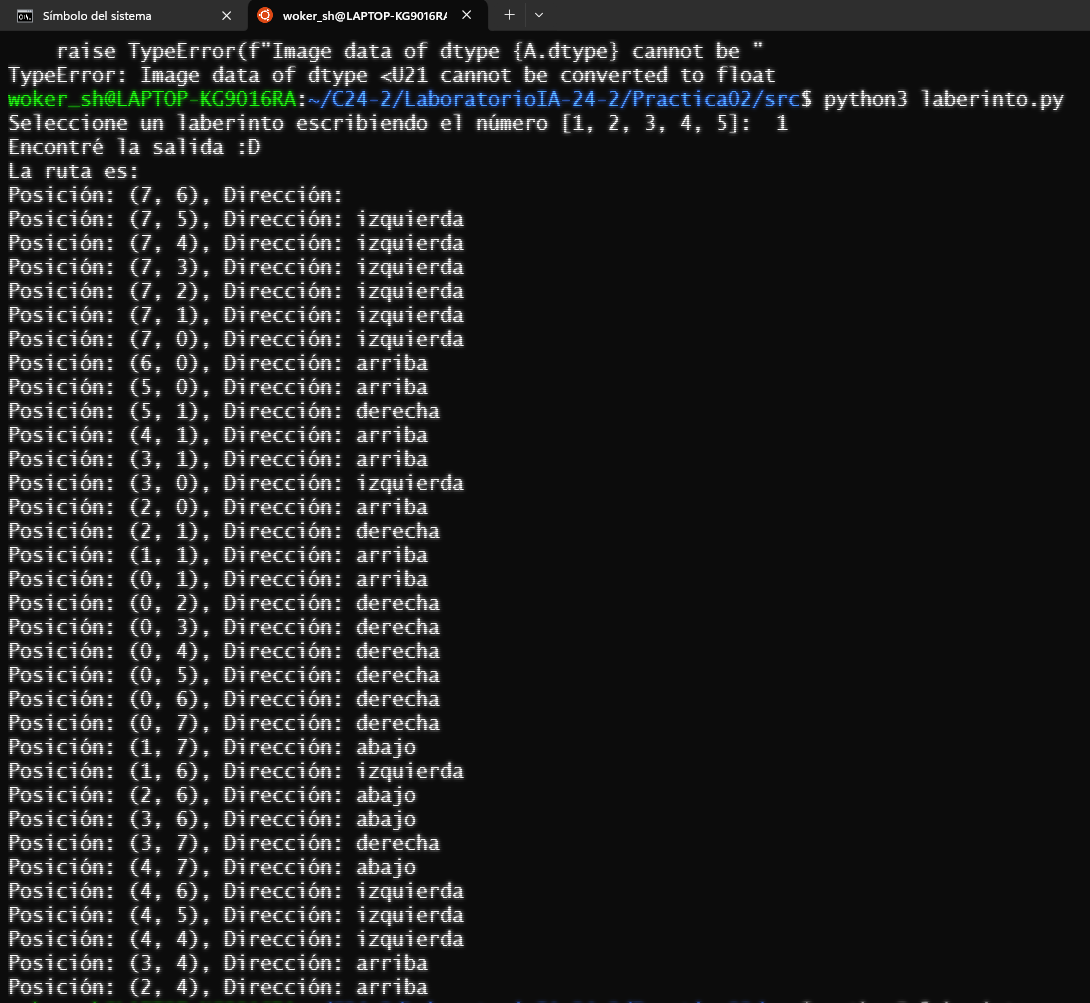
\includegraphics[scale = .5]{IMA/ejecuciones1.png}
\end{center}


\subsection*{Ejecución laberinto02 - laberinto05}
\begin{center}
    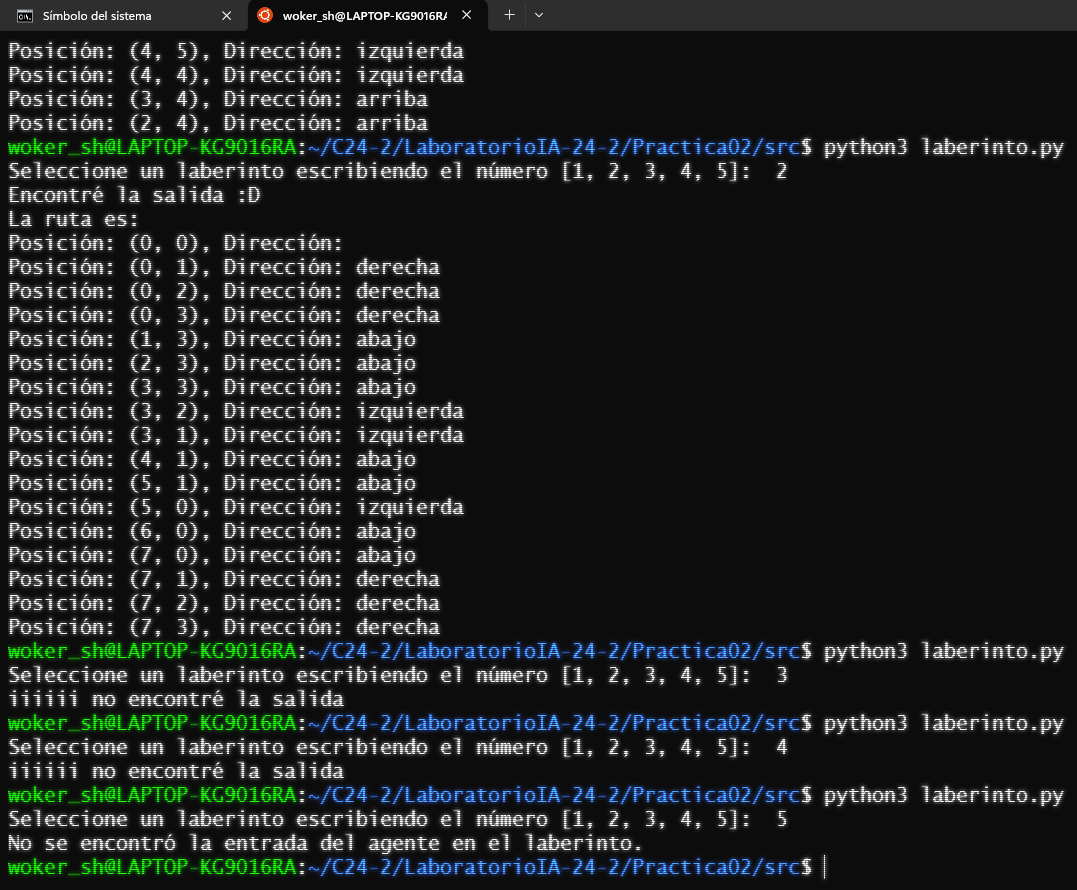
\includegraphics[scale = .5]{IMA/ejecuciones25.png}
\end{center}

Hemos realizado pruebas con dos entradas y dos salidas dentro del laberinto, los resultados son 
que si hay solución nos devuelve el recorrido que encuentre primero, es decir, la entrada que 
encuentre primero es la que toma así como la salida. 




% ----------------------|
% Referencias           |
% Forma de Compilar     |
% pdflatex main.tex     |
% biber main            |
% pdflatex main.tex     |
\newpage %              |
\thispagestyle{fancyref}
\printbibliography %    |
% ----------------------|

\end{document}%----------------------F I N DOCUMENTO---------------|
%------------------------------------------------------------------|
